\documentclass[pdf]{beamer}
\mode<presentation>{
	\usetheme{Ilmenau}

}
	\usecolortheme{beaver}
\usepackage[UTF8,indent]{ctexcap}
\usepackage{amssymb}
\usepackage{amsmath}
\usepackage{amsfonts}
%\usepackage{graphicx}
\usepackage{amsthm}
\usepackage{indentfirst}
\usepackage{enumerate}
\usepackage{extpfeil}
\usepackage{tikz-cd}

\usetikzlibrary {calc,positioning,shapes.misc,graphs,decorations.pathreplacing}
\usefonttheme[onlymath]{serif}

\numberwithin{equation}{section}

\theoremstyle{plain}
\newtheorem{proposition}[theorem]{Proposition}
\newtheorem{claim}[theorem]{Claim}
\newtheorem{defn}[theorem]{Definition}

\theoremstyle{plain}
\newtheorem{exercise}{Exercise}[section]


\theoremstyle{remark}
\newtheorem{remark}[theorem]{Remark}
\newtheorem{remarks}{Remarks}
\newtheorem{ex}[theorem]{Exercise}
\newtheorem{question}[theorem]{Question}

\newcommand*{\thick}[1]{\text{\boldmath$#1$}}
\newcommand*{\cir}[1]{\;$\ding{19#1}$\;}%临时使用
\newcommand*{\norm}[1]{\lVert#1\rVert}

\DeclareMathOperator{\supp}{supp}
\DeclareMathOperator{\dist}{dist}
\DeclareMathOperator{\vol}{vol}
\DeclareMathOperator{\diag}{diag}
\DeclareMathOperator{\tr}{tr}
\DeclareMathOperator{\Proj}{\operatorname{Proj}}
\newcommand*{\bigchi}{\mbox{\Large$\chi$}}% big chi
\setlength{\parindent}{2em}
\newcommand{\character}[2]{\left[\begin{array}{c}{#1} \\ {#2}\end{array}\right]}
\newcommand{\normalcharacter}{\character{\epsilon}{\epsilon'}}

\setbeamertemplate{caption}[numbered]
% 设置图形文件的搜索路径
\graphicspath{{figures/}}
\title[本科毕业论文答辩]{模形式和五次方程的解}
\author[周潇翔]{周潇翔\newline \newline 指导老师:许金兴}
\institute[USTC]{University of Science and Technology of China}
\date{\today}
\subject{模形式和五次方程的解}
\keywords{正多面体,\enskip 分歧覆叠,\enskip 预解式,\enskip 求根公式,\enskip 模形式,\enskip Theta函数,\enskip Klein四次曲线}
\tikzset{
	invisible/.style={opacity=0,text opacity=0},
	visible on/.style={alt=#1{}{invisible}},
	alt/.code args={<#1>#2#3}{%
		\alt<#1>{\pgfkeysalso{#2}}{\pgfkeysalso{#3}} % \pgfkeysalso doesn't change the path
	},
}
\setbeamercolor{section number projected}{fg=white!90!blue, bg=red!90!black}
\setbeamercolor{block body}{fg=black,bg=gray!10}
\setbeamercolor{block title}{fg=white, bg=red!64!black}


\setbeamertemplate{headline}{
	\begin{beamercolorbox}[wd=\paperwidth,ht=2.5ex,dp=1.125ex]{section in head/foot}%
		\hspace{3ex}{\insertsectionhead}
	\end{beamercolorbox}
%	\begin{beamercolorbox}[ht=2.5ex,dp=1.125ex,leftskip=.3cm,rightskip=.3cm plus1fil]{subsection in head/foot}
%		\usebeamerfont{subsection in head/foot}\insertsubsectionhead
%\end{beamercolorbox}
}%删除点

\begin{document}
	\setbeamercovered{transparent}
	\begin{frame}
\titlepage
\end{frame}

\begin{frame}{目录}
\tableofcontents[hideallsubsections]
\end{frame}
\section{正二十面体方程}
\begin{frame}{目录}
\tableofcontents[currentsection,hideallsubsections]
\end{frame}
	\begin{frame}[label=flowchart233,fragile]
\fontencoding{T1}\fontfamily{ptm}
	\setbeamercovered{invisible}
\begin{tikzpicture}[
double={blue!10}, double distance between line centers=3pt,
node distance=15mm,
terminal/.style={
	% The shape:
	rectangle,minimum size=6mm, minimum width=10mm,rounded corners=0mm,
	% The rest
	thick,draw=violet!50,
	top color=white,bottom color=violet!20,
	font=\ttfamily},
smaller/.style={
	% The shape:
	rectangle,minimum size=4mm,rounded corners=0mm,
	% The rest
	thick,draw=red!50,
	top color=white,bottom color=red!20,
	font=\ttfamily},
every new ->/.style={shorten >=1pt},
>={Implies[fill=blue!80]},thick,blue!90,text=black,
%arrows = {-Latex[length=5pt 3 0]}
]

\node (ratfct) [terminal, visible on=<11->] {有理函数};
%\node[smaller,right=of ratfct,yshift=-.45cm,xshift=1cm,font=\footnotesize, visible on=<15->]{扩张};
\node (fctfield) [terminal,right=of ratfct, visible on=<13->] {函数域};
%\node[smaller,right=of fctfield,yshift=-.45cm,xshift=1.8cm,font=\footnotesize, visible on=<15->]{子群};
\node (group) [terminal,right=of fctfield,xshift=1cm, visible on=<6->] {群} ;
\node[smaller,below=of fctfield,yshift=-.49cm,xshift=1cm,font=\footnotesize, visible on=<9->]{\hyperlink{covering<1>}{分歧覆叠}};
\node (RS) [terminal,below=of fctfield, visible on=<8->] {\hyperlink{RS<1>}{Riemann面}};
\node (sym) [terminal,below=of group, visible on=<4->] {对称性};
\node (poly) [terminal,below=of sym, visible on=<2->] {正多面体};
\path (fctfield) edge [->,double, visible on=<14->]node[above, visible on=<14->]{\small PET} (ratfct);
\path (fctfield) edge [<->,double, visible on=<12->]node[above, visible on=<12->]{\small Galois} (group);
\path (fctfield) edge [<->,double, visible on=<14->] (RS);
\path (group) edge [<->,double, visible on=<5->] (sym);
\path (poly) edge [<->,double, visible on=<3->] (sym);
\path (group) edge [->,double, visible on=<7->] (RS);
\path (RS) edge [->,double, visible on=<10->] (ratfct);
\draw[black,dashed] (-2.5,-1.5)--(8,-1.5);
\draw (-2,-1.5) node[anchor=south] {代数};
\draw (-2,-1.5) node[anchor=north] {几何};
%\path (shier) edge [<->,double]node[left]{\parbox{1.5cm}{\small 辅助方程}} ($(Bri1.north)+(10mm,0)$);
%\path ($(Bri1.south)+(10mm,0)$) edge [<->,double]node[left]{\parbox{2.5cm}{\small Tschirnhaus变换}} (qua);
%\path (jie.south west) edge [<->,double]node[right]{\parbox{1.5cm}{\small J-B约化}} (qua.north east);
\end{tikzpicture}
\only<14>{
	\begin{minipage}[t]{.75\textwidth}
		\vspace{-2cm}
		\begin{theorem}[本原元定理(PET)]
			域$\mathbb{C}(x)$的有限扩域$E$是单扩域,即,存在$y \in E$使得$E =\mathbb{C}(x)(y)$.
		\end{theorem}
		
	\end{minipage}
}
\only<15>{
	\begin{minipage}[t]{.75\textwidth}
		\vspace{-1.7cm}
		\begin{equation*}
		\begin{array}{ccc}
		\Gamma_1 &\subseteq& \Gamma_2\\
		\mathbb{PC}^1/\Gamma_1& \longrightarrow& \mathbb{PC}^1/\Gamma_2\\
		\mathcal{M}(\mathbb{PC}^1/\Gamma_1)& \supseteq& \mathcal{M}(\mathbb{PC}^1/\Gamma_2)
		\end{array}
		\end{equation*}	
	\end{minipage}
}
\only<6-13>{
	\begin{minipage}[t]{.75\textwidth}
		\vspace{-1.7cm}
		$$\uncover<13->{\mathcal{M}(}
		\uncover<8->{\mathbb{PC}^1/\Gamma}
		\uncover<13->{)} 
		\uncover<12->{\Longleftrightarrow} \Gamma$$
		\vspace{-0.5cm}
		$$\uncover<9->{\varPhi:\mathbb{PC}^1\xtwoheadrightarrow{}}
		\uncover<8->{\mathbb{PC}^1/\Gamma\overset{\sim}{\longrightarrow}\mathbb{PC}^1}$$		
	\end{minipage}
}
\end{frame}


%\begin{frame}{正十二面体群$\Gamma_{(2,3,5)} \cong A_5$}
%\begin{columns}
%	\begin{column}{0.7\textwidth}
%		\begin{itemize}[<+->]
%			\item 图\ref{eg:fig1}给出$\Gamma_{(2,3,5)}$的一个12阶子群$A_4$;
%			%这里子群不是正方体的自同构群
%			\item 不同的正方体给出不同且互相共轭的12阶子群;
%			
%			\item $\Gamma_{(2,3,5)}$中的元素给出5个正方体的置换,即群同态$$\alpha:\Gamma_{(2,3,5)}\longrightarrow S_5.$$
%			易验证$\ker(\alpha)=\{Id\}$, $Im(\alpha)=A_5$.因此$\Gamma_{(2,3,5)}\cong A_5$.
%			
%		\end{itemize}
%	\end{column}
%	\begin{column}{0.3\textwidth}
%		\begin{figure}[ht]
%			\centering
%			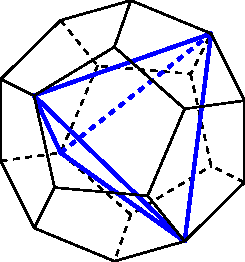
\includegraphics[scale=0.6]{poly/poly14.pdf}
%			\caption{嵌套正多面体}
%			\label{eg:fig1}
%		\end{figure}
%	\end{column}
%\end{columns}
%\end{frame}

%	\begin{frame}{多面体对应图像:正八面体/立方体}
%%%等待拍照???
%\begin{figure}[ht]
%	\centering
%	
\includegraphics[width=.45\textwidth]{fromweb/Gamma234.png}
%\end{figure}
%\end{frame}

%		\begin{frame}{符号:$\Gamma_{(v_1,v_2,v_3)}$}
%\centering
%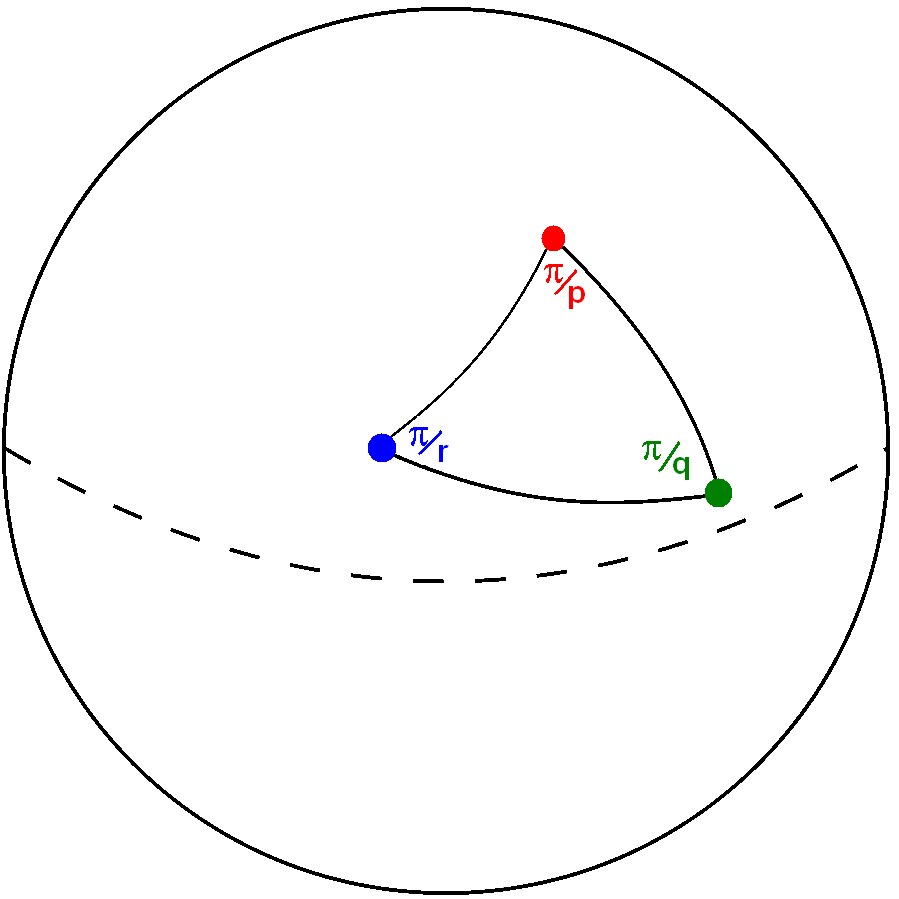
\includegraphics[scale=0.2]{fromweb/Schwarz_triangle.png}
%\end{frame}

%	\begin{frame}{任务}
%\hspace{-2em}
%$$\varPhi:\mathbb{PC}^1\xtwoheadrightarrow{}\mathbb{PC}^1/\Gamma\overset{\sim}{\longrightarrow}\mathbb{PC}^1$$

%\begin{itemize}
%	\item \alert{给出$\varPhi$的表达式;}
%	\item 描述$\mathbb{PC}^1/\Gamma$上的亚纯函数;
%	\item<0> 描述$\varPhi^{-1}$.
%\end{itemize}
%\end{frame}
%
%

%\begin{frame}{正多面体方程}
%	\begin{table}[ht]
%	\centering
%	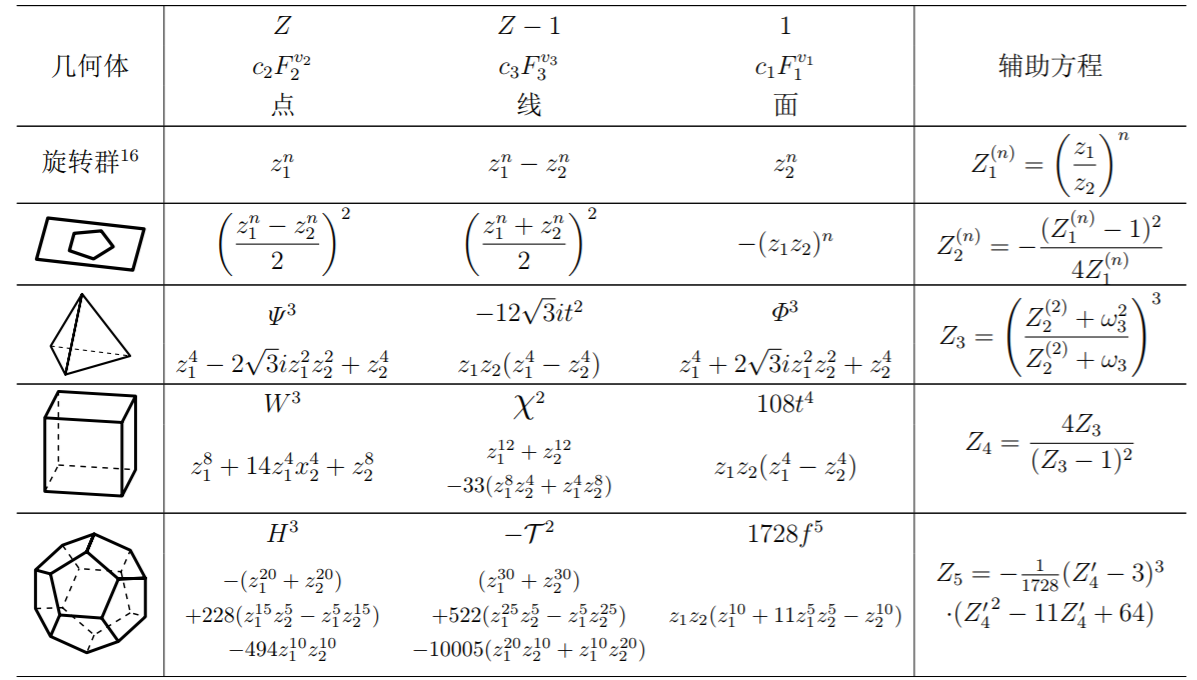
\includegraphics[width=0.9\textwidth]{snip/eqpoly.png}
%	\caption{正多面体对应方程}
%	\label{tb:equations}
%\end{table}
%\end{frame}
%	\begin{frame}[<+->]{任务}
%\hspace{-2em}
%$$\varPhi:\mathbb{PC}^1\xtwoheadrightarrow{}\mathbb{PC}^1/\Gamma\overset{\sim}{\longrightarrow}\mathbb{PC}^1$$
%对于正十二面体,
%\begin{itemize}
%	\item 给出$\varPhi$的表达式:
%	$$\varPhi=\frac{H^{\,3}}{1728f^{\,5}}$$
%	\item 描述$\mathbb{PC}^1/\Gamma$上的亚纯函数:
%	$$\mathcal{M}(\mathbb{PC}^1/\Gamma)=\mathbb{C}(\varPhi)$$
%	\item \alert<3>{描述$\varPhi^{-1}$.}
%\end{itemize}
%\end{frame}
%	\begin{frame}{任务}
%$$\varPhi:\mathbb{PC}^1\xtwoheadrightarrow{}\mathbb{PC}^1/\Gamma\overset{\sim}{\longrightarrow}\mathbb{PC}^1$$
%\begin{itemize}
%	\item 给出$\varPhi$的表达式;
%	\item 描述$\mathbb{PC}^1/\Gamma$上的亚纯函数;
%	\item \alert<1>{描述$\varPhi^{-1}$.}
%	\begin{itemize}
%		\item\alert<1>{复分析视角:多值函数;}
%		\item<0> 近世代数视角:预解式.
%	\end{itemize}
%\end{itemize}
%\end{frame}

	\begin{frame}[label=invarient2]{一些结论}
\hspace{-2em}
$$\varPhi:\mathbb{PC}^1\xtwoheadrightarrow{}\mathbb{PC}^1/\Gamma\overset{\sim}{\longrightarrow}\mathbb{PC}^1$$
对于正十二面体,
\begin{itemize}[<+->]
	\item $\varPhi$的表达式: $\, $ \hyperlink{invarient1}{\beamergotobutton{process}}
	$$\varPhi=\frac{H^{\,3}}{1728f^{\,5}}=\frac{\left\{-(z^{20}+1)+228(z^{15}-z^5)-494z^{10}\right\}^3}{1728\left\{z(z^{10}+11z^5-1)\right\}^5}$$
	\item $\mathbb{PC}^1/\Gamma$上的亚纯函数:
	$$\mathcal{M}(\mathbb{PC}^1/\Gamma)=\mathbb{C}(\varPhi)$$
	\item 可以分别从复分析和近世代数的角度描述$\varPhi^{-1}$.
\end{itemize}
\end{frame}
	\begin{frame}{正二十面体方程}
\begin{defn}
	称正二十面体方程为如下关于$z$的多项式方程
	$$H(z)^3-1728\varPhi_0 f(z)^5=0$$
	这等价于方程$\varPhi(z)=\varPhi_0$.
\end{defn}
\end{frame}
%\subsection{复分析视角:多值函数}
%	\begin{frame}{多值函数}
%$$\hspace{-2.5cm}\varPhi^{-1}\colon\hspace{1cm} \mathbb{PC}^1/\Gamma\hspace{2cm} \longrightarrow \hspace{2cm}\mathbb{PC}^1$$
%\begin{figure}[ht]
%	
%	\raisebox{-1.5cm}{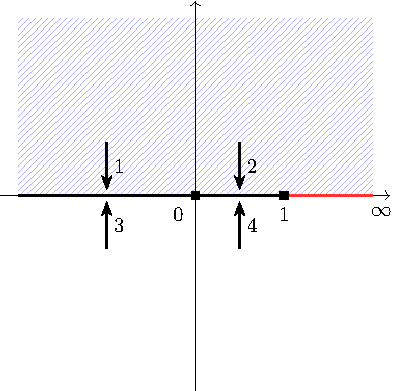
\includegraphics[scale=0.5]{pic/halfspace.pdf}} $\qquad\longrightarrow\qquad$ 	\only<1>{\raisebox{-0.75cm}{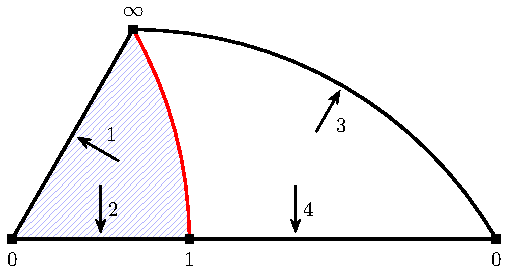
\includegraphics[scale=0.5]{pic/halfspace2.pdf}\hspace{-1.1cm}}	
%	}\only<2>{
%		\raisebox{-1cm}{
\includegraphics[scale=0.12]{fromweb/Gamma234.png}}\hspace{.6cm}
%	}
%	\label{pic:Ctriangle}
%\end{figure}
%\end{frame}

%	\begin{frame}{接下来的相关工作}
%我们可以得到
%\begin{itemize}[<+->]
%	\item 单值解析分支的表达式;
%	\item 不同单值解析分支之间的关系;
%	\item 单值解析分支满足的常微分方程.
%\end{itemize}
%\end{frame}
\section{模方程}
\begin{frame}{目录}
\tableofcontents[currentsection,hideallsubsections]
\end{frame}

%	\begin{frame}{预解式}
%时间关系跳过...
%\end{frame}
	\begin{frame}[fragile]{符号解释}
	\begin{itemize}
		\item $SL_2(\mathbb{Z}):=$行列式为1的整系数矩阵构成的群;
		\item $\displaystyle\Gamma(N):=\left\{ \begin{pmatrix}
		a &b \\ c & d
		\end{pmatrix} \in SL_2(\mathbb{Z}) \;\middle|\; \begin{pmatrix}
		a &b \\ c & d
		\end{pmatrix} \equiv \begin{pmatrix}
		1 &0 \\ 0 & 1
		\end{pmatrix} \mod N  \right\};$
		\item 特别地, $\Gamma(1)=SL_2(\mathbb{Z})$;
		\item $\mathcal{H}:=$上半平面;
		\item $\mathcal{H}^*:=\mathcal{H} \sqcup \mathbb{PQ}^1$.
	\end{itemize}



\end{frame}
%\section{模空间与$\theta$函数}
%\begin{frame}{目录}
%\tableofcontents[currentsection,hideallsubsections]
%\end{frame}
\begin{frame}{模空间}
\begin{columns}
	\begin{column}{0.5\textwidth}
		\begin{figure}[ht]
			\centering
			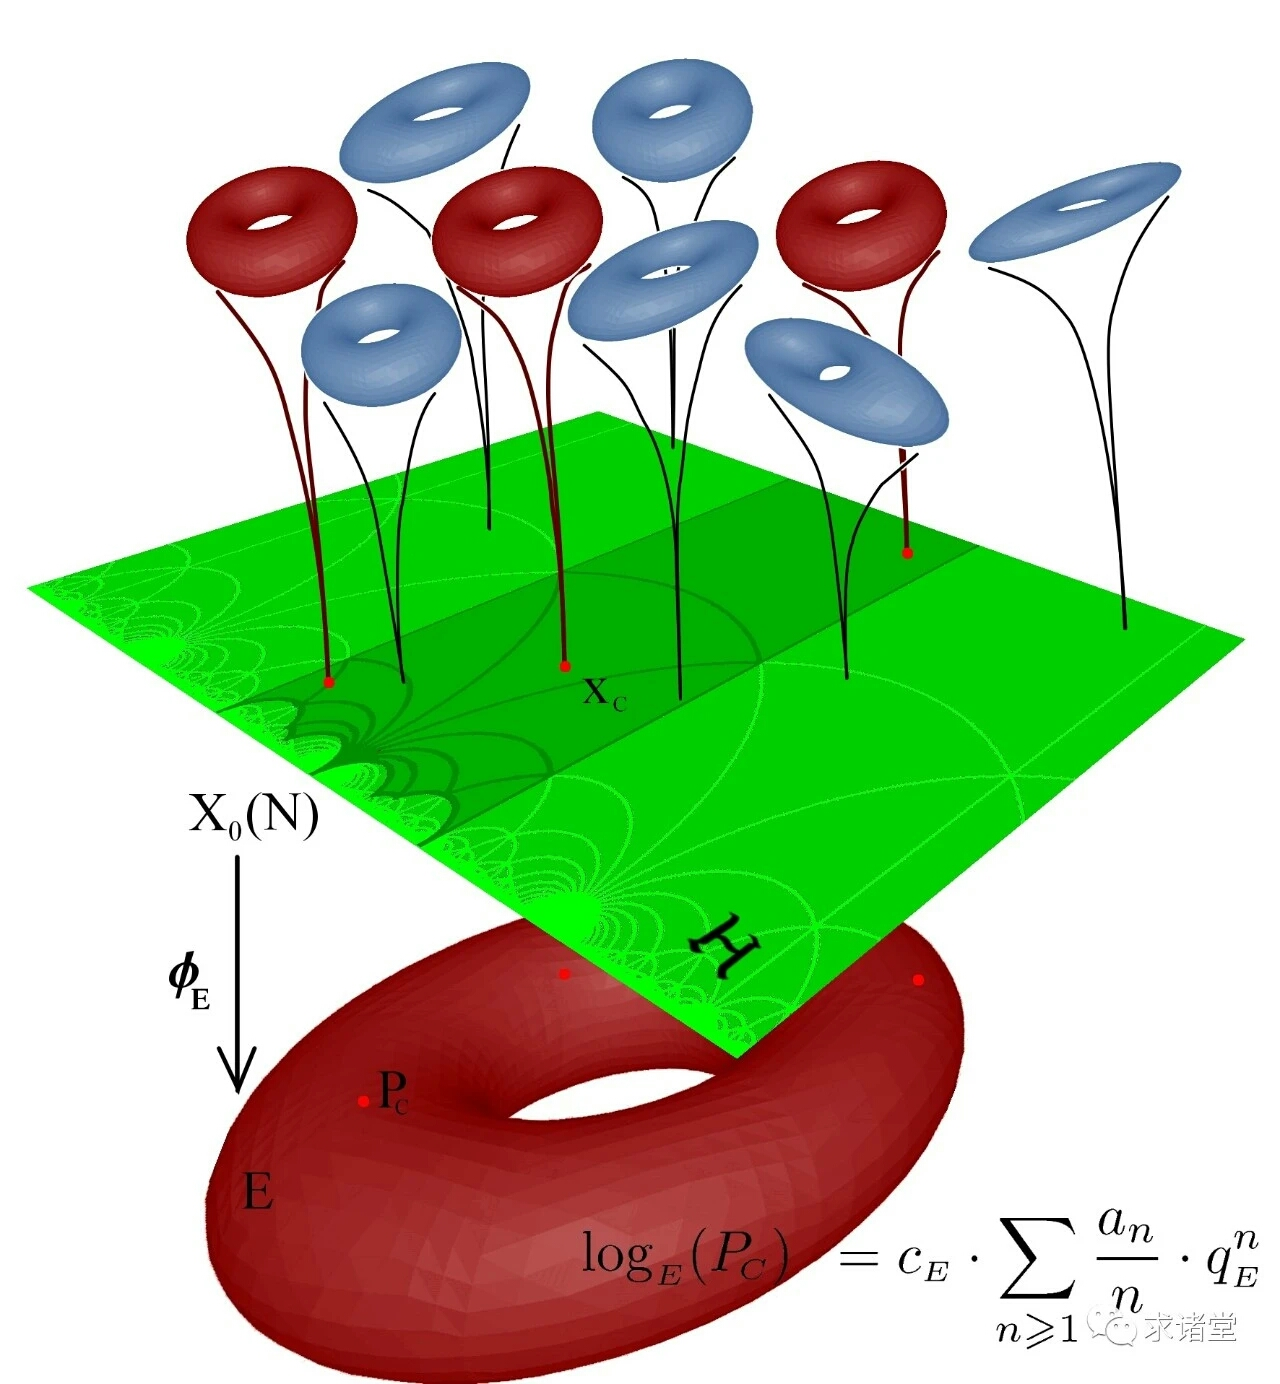
\includegraphics[height=.7\textheight]{fromweb/modularspace.jpg}
		\end{figure}
	\end{column}
	\begin{column}{0.5\textwidth}
		\begin{itemize}
			\item $\mathcal{H}/\Gamma(1)$:分类复环面;
			\item $\mathcal{H}/\Gamma(N)$:分类复环面+复环面上的级结构.
		\end{itemize}
	\end{column}
\end{columns}
\end{frame}
	\begin{frame}[label=thereturn]{$\mathbb{C}/\Lambda$与$\mathcal{H}/SL_2(\mathbb{Z})$}
\begin{table}[ht]
	\centering
	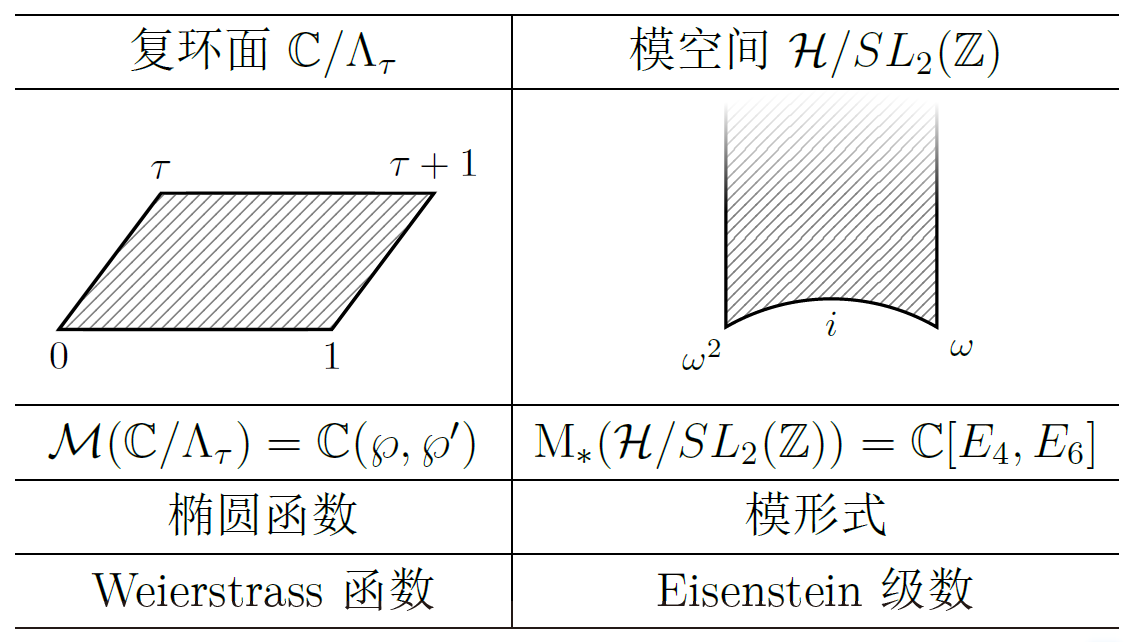
\includegraphics[width=0.8\textwidth]{snip/table-torus-moduli.png}
	\caption{复环面与模空间的比较}
	\label{tb:torus-moduli}
\end{table}
\hyperlink{thetafcts}{\beamergotobutton{$\theta$ functions}}
\end{frame}

\begin{frame}{$\mathcal{H}/\Gamma(5)$:基本区域}
%%插入N=5,N=7的图片
\begin{table}[ht]
	\centering
	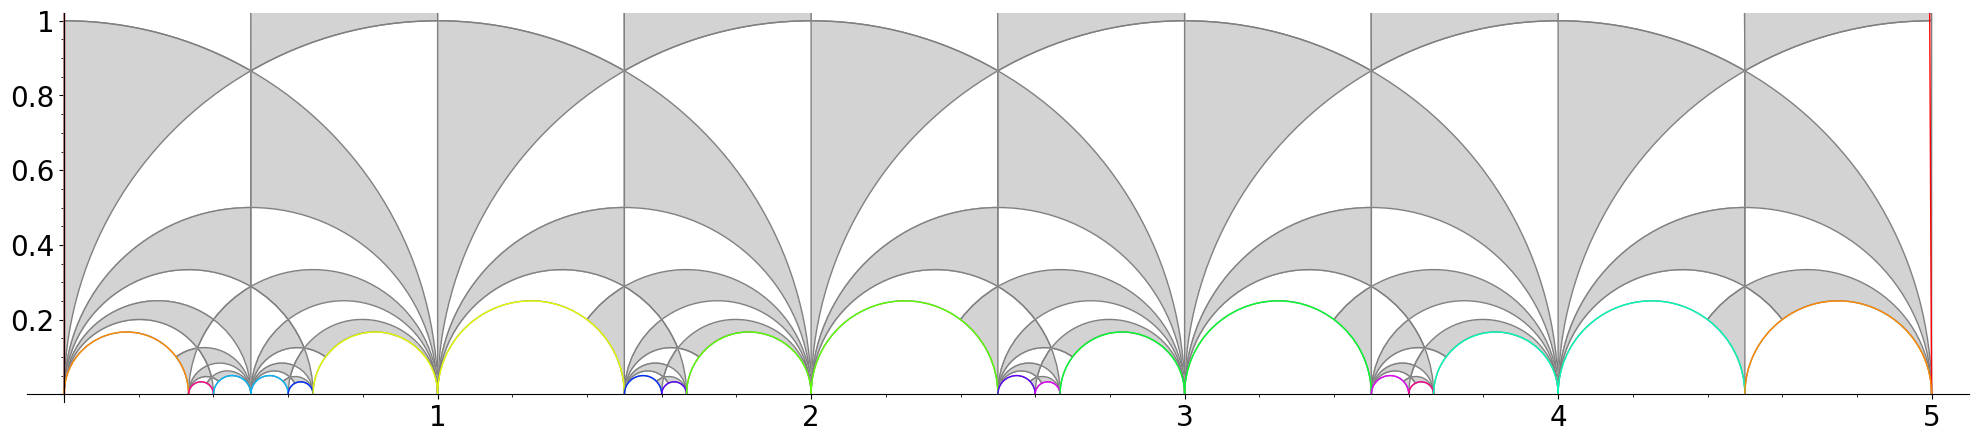
\includegraphics[width=1\textwidth]{sage/X(5).png}
	\caption{$\mathcal{H}/\Gamma(5)$的基本区域}
	
\end{table}

\end{frame}
\begin{frame}{$\mathcal{H}/\Gamma(5)$:紧化}
%%插入N=5,N=7的图片
\begin{table}[ht]
	\centering
	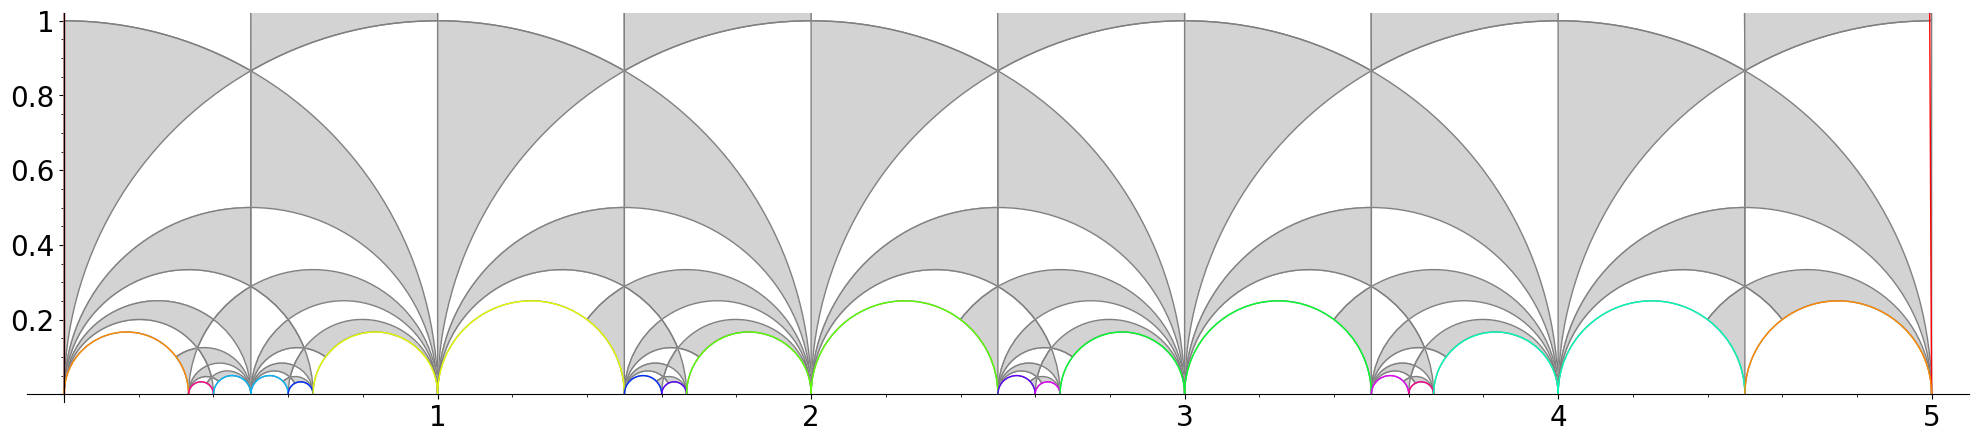
\includegraphics[width=1\textwidth]{sage/X(5).png}
\end{table}
$$\Downarrow \hat{j_5}$$
\begin{figure}[ht]
	\centering
	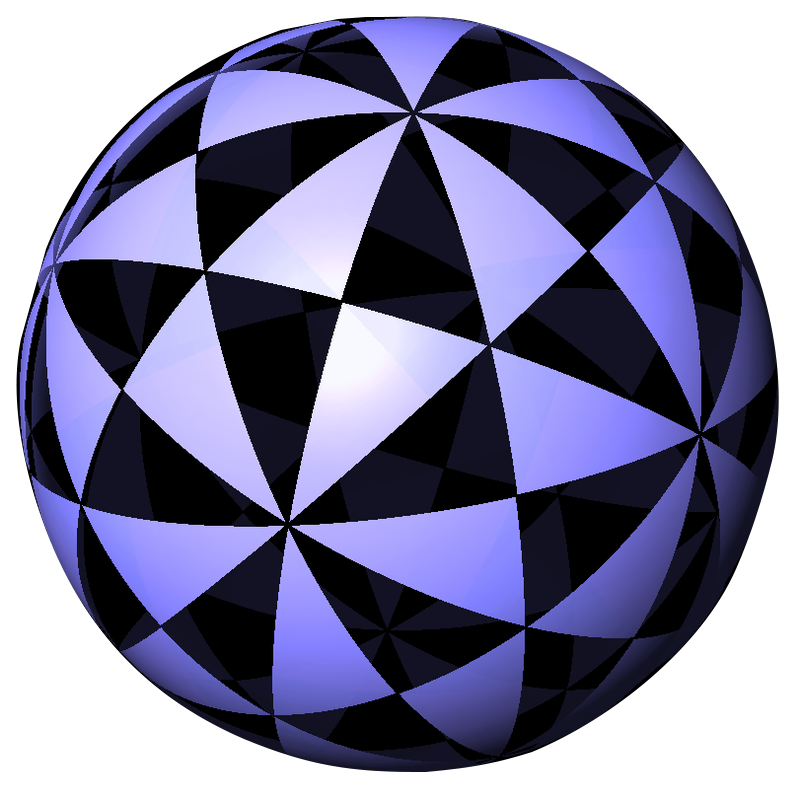
\includegraphics[width=.2\textwidth]{fromweb/Gamma235.png}
\end{figure}
\end{frame}

\begin{frame}{$\mathcal{H}/\Gamma(7)$:基本区域}
%%插入N=5,N=7的图片
\begin{table}[ht]
	\centering
	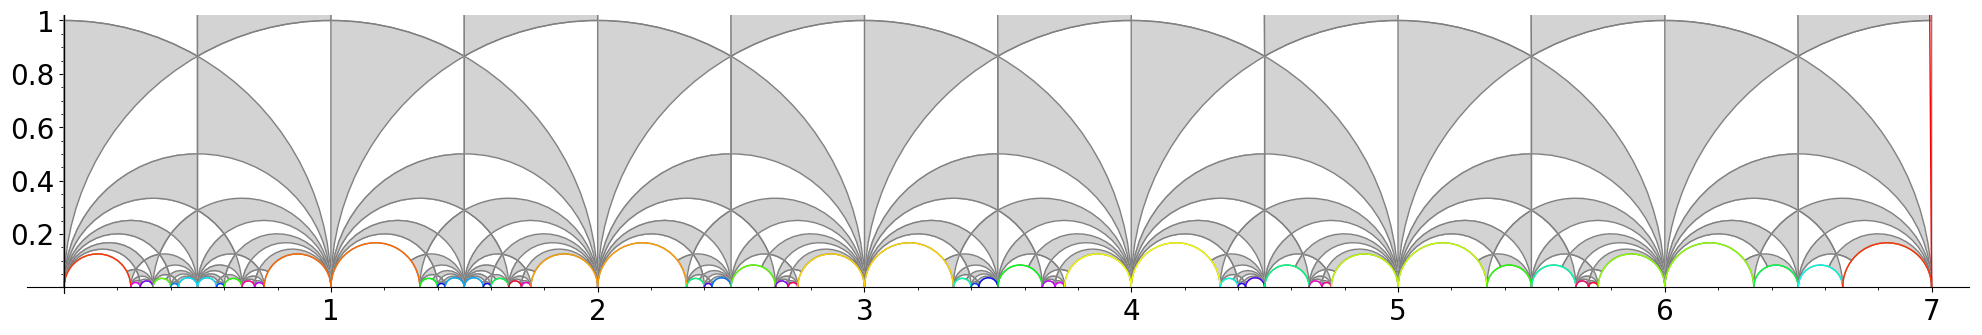
\includegraphics[width=1\textwidth]{sage/X(7).png}
	\caption{$\mathcal{H}/\Gamma(7)$的基本区域}
\end{table}

\end{frame}
\begin{frame}{$\mathcal{H}/\Gamma(7)$:Klein四次曲线}
%%插入N=5,N=7的图片
\begin{table}[ht]
	\centering
	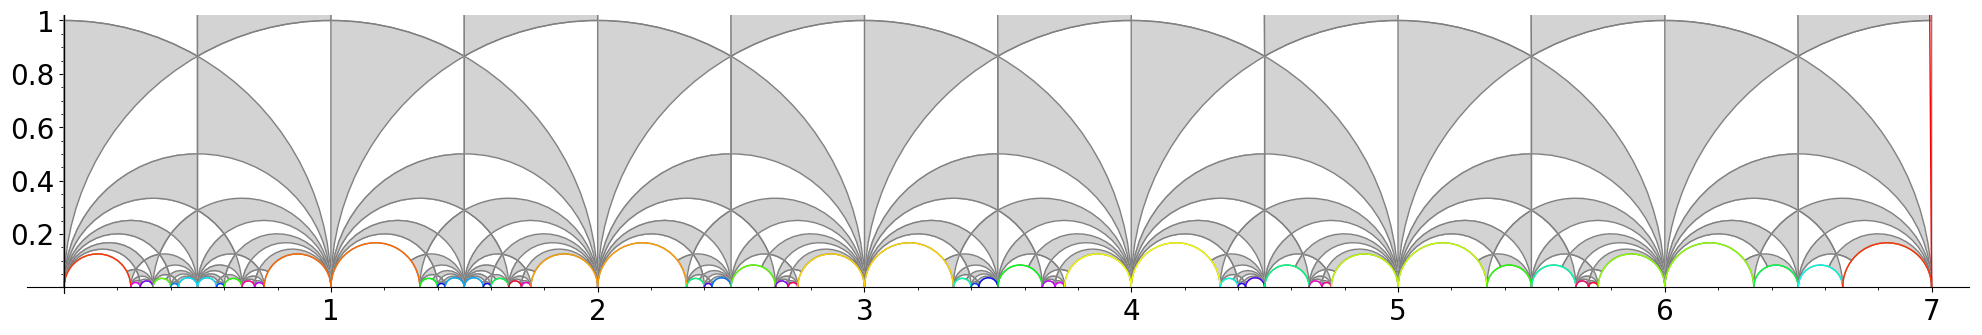
\includegraphics[width=1\textwidth]{sage/X(7).png}
\end{table}
$$\Downarrow \Phi$$

\only<1>{\begin{figure}[ht]
		\centering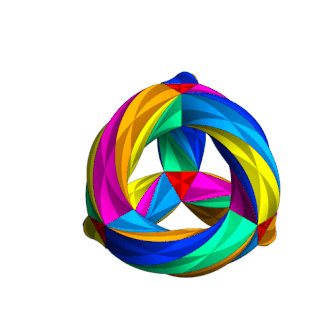
\includegraphics[width=.37\textwidth,clip=true,trim=40pt 10pt 0pt 40pt]{gif/images/Kleincurve-0.png}\end{figure}}
%\only<2>{\begin{figure}[ht]
%		\centering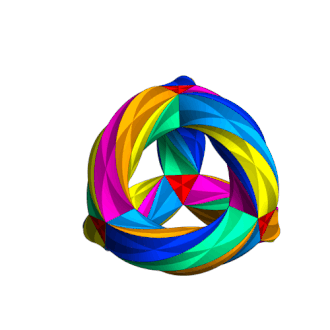
\includegraphics[width=.37\textwidth,clip=true,trim=40pt 10pt 0pt 40pt]{gif/images/Kleincurve-1.png}\end{figure}}
%\only<3>{\begin{figure}[ht]
%		\centering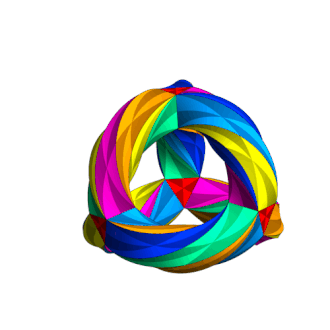
\includegraphics[width=.37\textwidth,clip=true,trim=40pt 10pt 0pt 40pt]{gif/images/Kleincurve-2.png}\end{figure}}
%\only<4>{\begin{figure}[ht]
%		\centering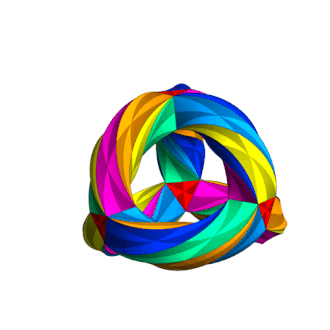
\includegraphics[width=.37\textwidth,clip=true,trim=40pt 10pt 0pt 40pt]{gif/images/Kleincurve-3.png}\end{figure}}
%\only<5>{\begin{figure}[ht]
%		\centering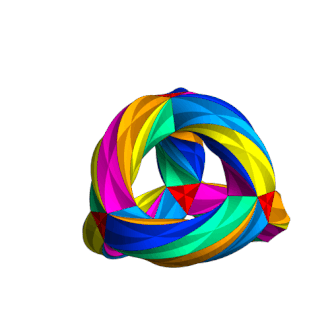
\includegraphics[width=.37\textwidth,clip=true,trim=40pt 10pt 0pt 40pt]{gif/images/Kleincurve-4.png}\end{figure}}
%\only<6>{\begin{figure}[ht]
%		\centering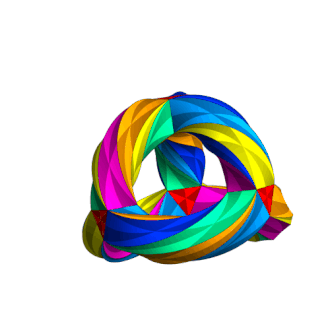
\includegraphics[width=.37\textwidth,clip=true,trim=40pt 10pt 0pt 40pt]{gif/images/Kleincurve-5.png}\end{figure}}
%\only<7>{\begin{figure}[ht]
%		\centering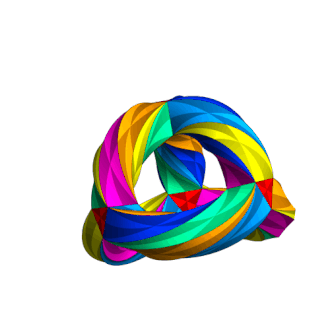
\includegraphics[width=.37\textwidth,clip=true,trim=40pt 10pt 0pt 40pt]{gif/images/Kleincurve-6.png}\end{figure}}
%\only<8>{\begin{figure}[ht]
%		\centering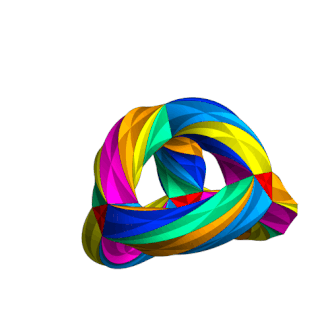
\includegraphics[width=.37\textwidth,clip=true,trim=40pt 10pt 0pt 40pt]{gif/images/Kleincurve-7.png}\end{figure}}
%\only<9>{\begin{figure}[ht]
%		\centering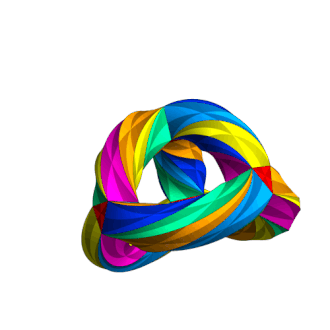
\includegraphics[width=.37\textwidth,clip=true,trim=40pt 10pt 0pt 40pt]{gif/images/Kleincurve-8.png}\end{figure}}
%\only<10>{\begin{figure}[ht]
%		\centering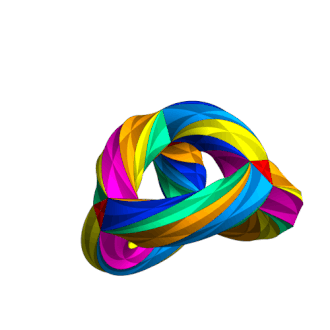
\includegraphics[width=.37\textwidth,clip=true,trim=40pt 10pt 0pt 40pt]{gif/images/Kleincurve-9.png}\end{figure}}
%\only<11>{\begin{figure}[ht]
%		\centering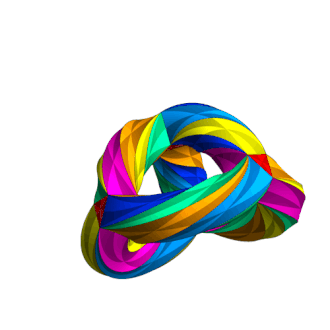
\includegraphics[width=.37\textwidth,clip=true,trim=40pt 10pt 0pt 40pt]{gif/images/Kleincurve-10.png}\end{figure}}
%\only<12>{\begin{figure}[ht]
%		\centering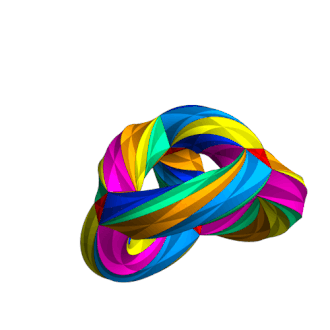
\includegraphics[width=.37\textwidth,clip=true,trim=40pt 10pt 0pt 40pt]{gif/images/Kleincurve-11.png}\end{figure}}
%\only<13>{\begin{figure}[ht]
%		\centering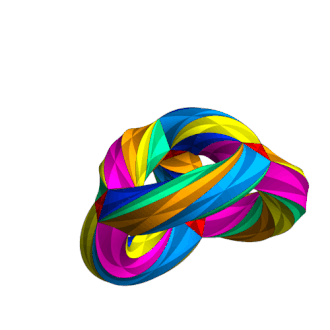
\includegraphics[width=.37\textwidth,clip=true,trim=40pt 10pt 0pt 40pt]{gif/images/Kleincurve-12.png}\end{figure}}
%\only<14>{\begin{figure}[ht]
%		\centering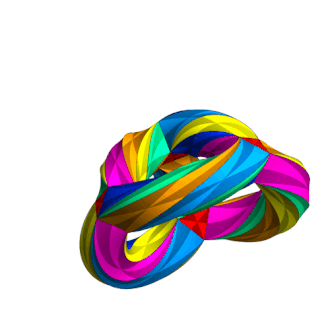
\includegraphics[width=.37\textwidth,clip=true,trim=40pt 10pt 0pt 40pt]{gif/images/Kleincurve-13.png}\end{figure}}
%\only<15>{\begin{figure}[ht]
%		\centering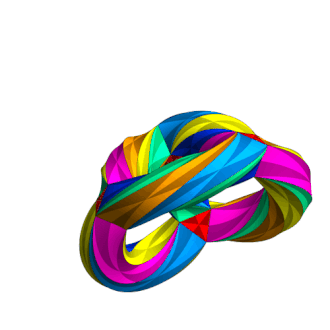
\includegraphics[width=.37\textwidth,clip=true,trim=40pt 10pt 0pt 40pt]{gif/images/Kleincurve-14.png}\end{figure}}
%\only<16>{\begin{figure}[ht]
%		\centering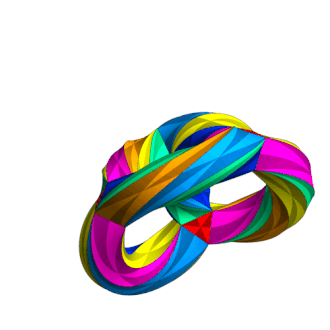
\includegraphics[width=.37\textwidth,clip=true,trim=40pt 10pt 0pt 40pt]{gif/images/Kleincurve-15.png}\end{figure}}
%\only<17>{\begin{figure}[ht]
%		\centering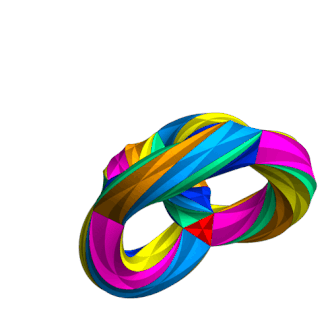
\includegraphics[width=.37\textwidth,clip=true,trim=40pt 10pt 0pt 40pt]{gif/images/Kleincurve-16.png}\end{figure}}
%\only<18>{\begin{figure}[ht]
%		\centering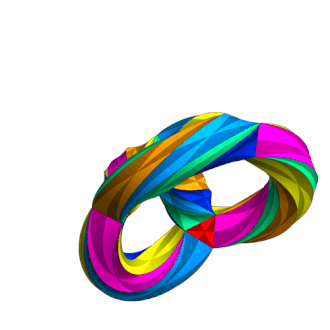
\includegraphics[width=.37\textwidth,clip=true,trim=40pt 10pt 0pt 40pt]{gif/images/Kleincurve-17.png}\end{figure}}
%\only<19>{\begin{figure}[ht]
%		\centering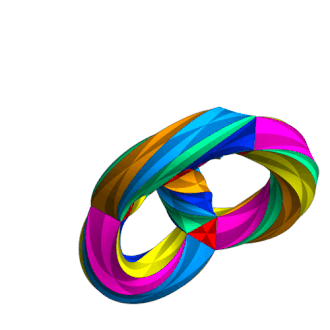
\includegraphics[width=.37\textwidth,clip=true,trim=40pt 10pt 0pt 40pt]{gif/images/Kleincurve-18.png}\end{figure}}
%\only<20>{\begin{figure}[ht]
%		\centering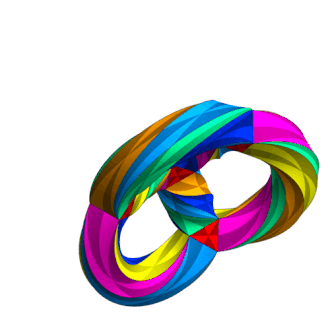
\includegraphics[width=.37\textwidth,clip=true,trim=40pt 10pt 0pt 40pt]{gif/images/Kleincurve-19.png}\end{figure}}
%\only<21>{\begin{figure}[ht]
%		\centering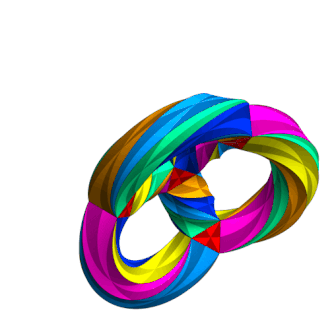
\includegraphics[width=.37\textwidth,clip=true,trim=40pt 10pt 0pt 40pt]{gif/images/Kleincurve-20.png}\end{figure}}
%\only<22>{\begin{figure}[ht]
%		\centering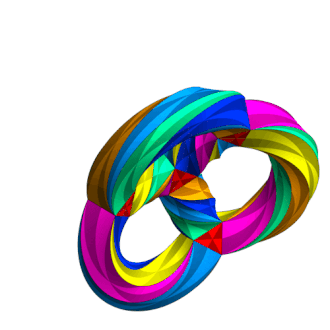
\includegraphics[width=.37\textwidth,clip=true,trim=40pt 10pt 0pt 40pt]{gif/images/Kleincurve-21.png}\end{figure}}
%\only<23>{\begin{figure}[ht]
%		\centering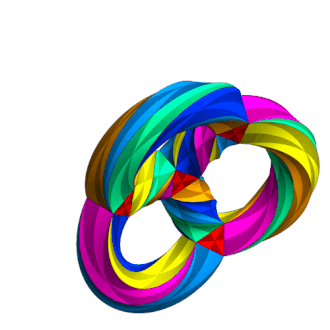
\includegraphics[width=.37\textwidth,clip=true,trim=40pt 10pt 0pt 40pt]{gif/images/Kleincurve-22.png}\end{figure}}
%\only<24>{\begin{figure}[ht]
%		\centering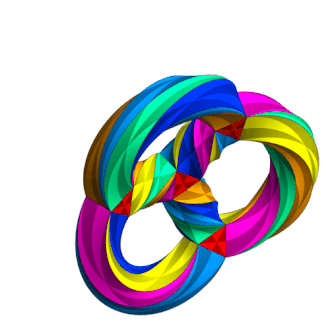
\includegraphics[width=.37\textwidth,clip=true,trim=40pt 10pt 0pt 40pt]{gif/images/Kleincurve-23.png}\end{figure}}
%\only<25>{\begin{figure}[ht]
%		\centering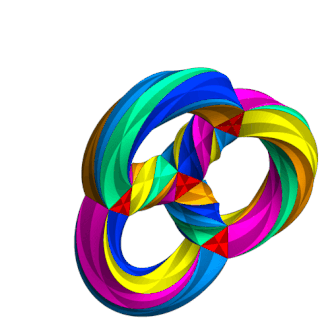
\includegraphics[width=.37\textwidth,clip=true,trim=40pt 10pt 0pt 40pt]{gif/images/Kleincurve-24.png}\end{figure}}
%\only<26>{\begin{figure}[ht]
%		\centering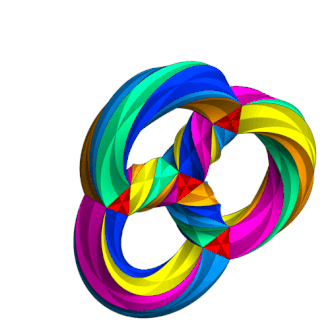
\includegraphics[width=.37\textwidth,clip=true,trim=40pt 10pt 0pt 40pt]{gif/images/Kleincurve-25.png}\end{figure}}
%\only<27>{\begin{figure}[ht]
%		\centering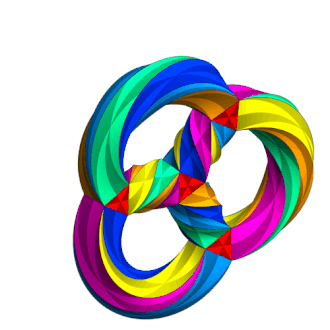
\includegraphics[width=.37\textwidth,clip=true,trim=40pt 10pt 0pt 40pt]{gif/images/Kleincurve-26.png}\end{figure}}
%\only<28>{\begin{figure}[ht]
%		\centering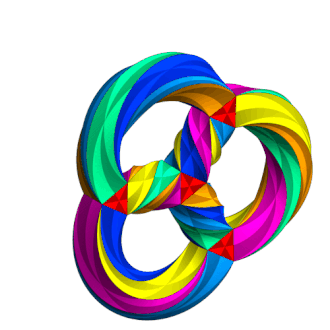
\includegraphics[width=.37\textwidth,clip=true,trim=40pt 10pt 0pt 40pt]{gif/images/Kleincurve-27.png}\end{figure}}
%\only<29>{\begin{figure}[ht]
%		\centering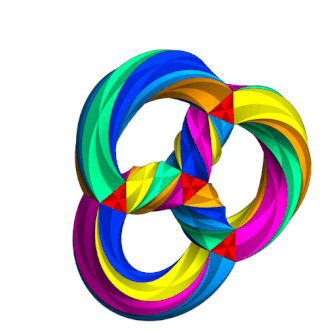
\includegraphics[width=.37\textwidth,clip=true,trim=40pt 10pt 0pt 40pt]{gif/images/Kleincurve-28.png}\end{figure}}
%\only<30>{\begin{figure}[ht]
%		\centering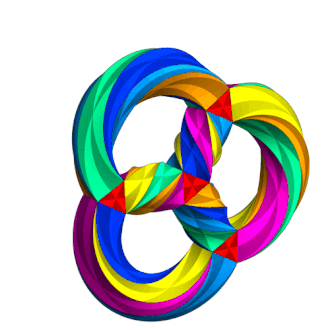
\includegraphics[width=.37\textwidth,clip=true,trim=40pt 10pt 0pt 40pt]{gif/images/Kleincurve-29.png}\end{figure}}
\only<2>{\begin{figure}[ht]
		\centering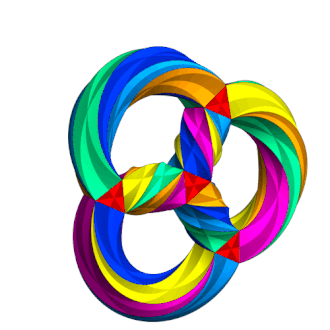
\includegraphics[width=.37\textwidth,clip=true,trim=40pt 10pt 0pt 40pt]{gif/images/Kleincurve-30.png}\end{figure}}
\end{frame}


%\begin{frame}{例:正十二面体对应的分歧覆叠}
%\hspace{-2em}
%$$\varPhi:\mathbb{PC}^1\xtwoheadrightarrow{}\mathbb{PC}^1/\Gamma\overset{\sim}{\longrightarrow}\mathbb{PC}^1$$
%
%\begin{figure}[ht]
%
%\begin{minipage}[t]{.34\textwidth}
%\vspace{0.1cm}
%%正十二面体
%\centering
%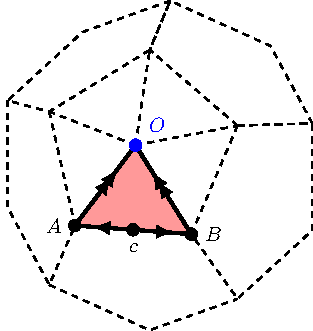
\includegraphics[width=2.25cm]{poly/poly4-2-3.pdf}
%
%\end{minipage}
%\begin{minipage}[t]{.64\textwidth}
%\vspace{0.1cm}
%\centering
%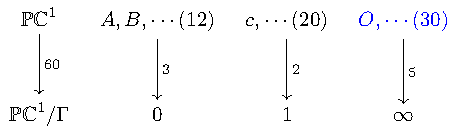
\includegraphics[scale=0.75]{commu/commu2-1-00.pdf}\\[0cm]
%在$0,1,\infty$处分歧,分歧指标为$(2,3,5)$
%\end{minipage}
%\label{pic:comm2-1}
%\end{figure}
%\end{frame}
%\begin{frame}{例:正十二面体对应的分歧覆叠}
%\hspace{-2em}
%$$\varPhi:\mathbb{PC}^1\xtwoheadrightarrow{}\mathbb{PC}^1/\Gamma\overset{\sim}{\longrightarrow}\mathbb{PC}^1$$
%\begin{figure}[ht]
%
%\begin{minipage}[t]{.34\textwidth}
%\vspace{0.1cm}
%%正十二面体
%\centering
%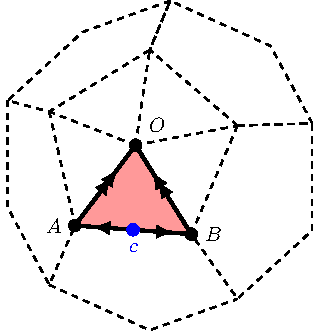
\includegraphics[width=2.25cm]{poly/poly4-2-2.pdf}
%
%\end{minipage}
%\begin{minipage}[t]{.64\textwidth}
%\vspace{0.1cm}
%\centering
%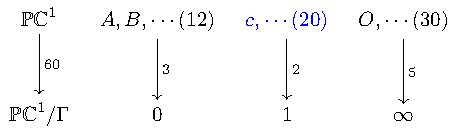
\includegraphics[scale=0.75]{commu/commu2-2-00.pdf}\\[0cm]
%在$0,1,\infty$处分歧,分歧指标为$(2,3,5)$
%\end{minipage}
%\label{pic:comm2-2}
%\end{figure}
%\end{frame}
%\begin{frame}{例:正十二面体对应的分歧覆叠}
%\hspace{-2em}
%$$\varPhi:\mathbb{PC}^1\xtwoheadrightarrow{}\mathbb{PC}^1/\Gamma\overset{\sim}{\longrightarrow}\mathbb{PC}^1$$
%\begin{figure}[ht]
%
%\begin{minipage}[t]{.34\textwidth}
%\vspace{0.1cm}
%%正十二面体
%\centering
%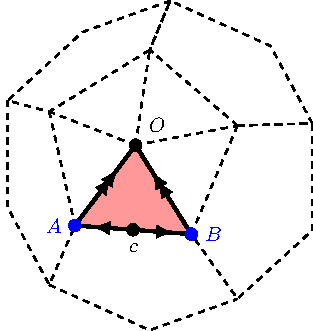
\includegraphics[width=2.25cm]{poly/poly4-2-1.pdf}
%
%\end{minipage}
%\begin{minipage}[t]{.64\textwidth}
%\vspace{0.1cm}
%\centering
%\includegraphics[scale=0.75]{commu/commu2-3-00.pdf}\\[0cm]
%在$0,1,\infty$处分歧,分歧指标为$(2,3,5)$
%\end{minipage}
%\label{pic:comm2-3}
%
%\end{figure}
%\hyperlink{flowchart233<9>}{\beamergotobutton{return}}
%\end{frame}
%\frame{\frametitle{$\mathcal{H}/\Gamma(N)$:基本区域}
%	\framezoom<1><2>[border](0cm,0cm)(4cm,1cm)
%	\hypersetup{linkbordercolor={red!70!black}}
%\begin{table}[ht]
%	\includegraphics[scale=0.2]{sage/X(7).png}
%	\caption{$\mathcal{H}/\Gamma(7)$的基本区域}
%\end{table}
%}%

\section{应用:解五次方程}
\begin{frame}{目录}
\tableofcontents[currentsection,hideallsubsections]
\end{frame}
\begin{frame}{流程图}
\begin{figure}[ht]
	\centering
	\fontencoding{T1}\fontfamily{ptm}
	\begin{tikzpicture}[
	double distance between line centers=3pt,
	node distance=15mm,
	terminal/.style={
		% The shape:
		rectangle,minimum size=6mm,rounded corners=3mm,
		% The rest
		very thick,draw=black!50,
		top color=white,bottom color=black!20,
		font=\ttfamily},
	every new ->/.style={shorten >=1pt},
	>={Implies},thick,black!50,text=black,
	%arrows = {-Latex[length=5pt 3 0]}
	]
	
	\node (mod) [terminal, visible on=<1->] {模方程$j(\tau)$的解};
	\node (shier) [terminal,below=of mod,yshift=0.5cm, visible on=<3->] {正二十面体方程$\varPhi(z)=\varPhi_0$的解};
	\node (Bri) [coordinate,below=of shier] {};
	\node (Bri1) [terminal,left=of Bri,xshift=1.7cm, visible on=<2->] {Brioschi预解式};
	\node (qua) [terminal,below=of Bri, visible on=<1->] {五次方程解};
	\node (jie) [terminal,right=of Bri1, visible on=<2->] {$x^5-x+\gamma=0$的解};
	\path (mod) edge [->,double, visible on=<4->] (shier);
	\path (shier) edge [<->,double, visible on=<3->]node[left, visible on=<3->]{\parbox{1.5cm}{\small 辅助方程}} ($(Bri1.north)+(10mm,0)$);
	\path ($(Bri1.south)+(10mm,0)$) edge [<->,double, visible on=<2->]node[left, visible on=<2->]{\parbox{2.5cm}{\small Tschirnhaus变换}} (qua);
	\path (jie.south west) edge [<->,double, visible on=<2->]node[right, visible on=<2->]{\parbox{1.5cm}{\small J-B约化}} (qua.north east);
	\end{tikzpicture}
\end{figure}
\end{frame}
\begin{frame}[label=flowchart1]{流程图}
\begin{columns}
\begin{column}{0.4\textwidth}
	\begin{figure}[ht]
		\centering
		\includegraphics[scale=0.7]{Flowchart/Mainflowchart-1.pdf}
	\end{figure}
\end{column}
\begin{column}{0.6\textwidth}
	\begin{figure}[ht]
		\centering
		\includegraphics[scale=0.7]{Flowchart/Mainflowchart-2-1.pdf}
	\end{figure}
\end{column}
\end{columns}
\hspace{-1cm}\hyperlink{fifth}{\beamergotobutton{more details}}
\end{frame}
	\begin{frame}[fragile]{模方程解正二十面体方程}
$$\text{记 \;}\Gamma(N):=\left\{ \begin{pmatrix}
a &b \\ c & d
\end{pmatrix} \in SL_2(\mathbb{Z}) \;\middle|\; \begin{pmatrix}
a &b \\ c & d
\end{pmatrix} \equiv \begin{pmatrix}
1 &0 \\ 0 & 1
\end{pmatrix} \mod N  \right\}$$
则有交换图
\only<1-2>{}
\begin{center}
	\begin{tikzcd}
		\mathcal{H}^* \arrow[r, "r"] & \mathcal{H}^*/\Gamma(5) \arrow[r, "\pi_1"] \arrow[d, "\hat{j}_5","\sim"'] & \mathcal{H}^*/\Gamma(1) \arrow[d, "\hat{j}","\sim"'] \\
		& \mathbb{PC}^1 \arrow[r, "\varPhi"]                                      & \mathbb{PC}^1/\Gamma                      
	\end{tikzcd}
\end{center}
$$\big(\Gamma(1)/\Gamma(5) \cong PSL_2(\mathbb{F}_5) \cong \Gamma\big)$$
\end{frame}
\begin{frame}{}
\centering \Huge
\emph{Thank You!}
\end{frame}
\begin{frame}{}
\begin{table}[th]
	\scalebox{1.5}{
	\begin{tabular}{c|c|c}
		\hline		
		截影 & 不变量 & 经典模形式:$\theta$函数\\
		\hline
		函数 & $\varPhi$ & $j,j_5$\\
		\hline
		空间 & $\mathbb{PC}^1/\Gamma$ & $\mathcal{H}^*/\Gamma(N)$\\
		\hline
	\end{tabular}
}
\end{table}
\end{frame}
%%%%%%%%%%%%%%%%%%%%%%%%%%%%%%%%%%%%%%%%%%%%%%%%%%%%%%%%%%%%%%%%%%%%%%%%%%
%预备军拾遗
\section*{拾遗}

\begin{frame}[label=fifth]{正多面体方程}
\begin{table}[ht]
	\centering
	\includegraphics[width=0.9\textwidth]{snip/eqpoly.png}
	\caption{正多面体对应方程}
	\label{tb:equations}
\end{table}
\end{frame}
\begin{frame}{辅助方程}
\begin{remarks}\
	\begin{itemize}
		\item 由于嵌入正十二面体的立方体为\textbf{倾斜放置},辅助方程为$Z_4'$,与$Z_4$相差一个分式线性变换.倾斜的立方体对应的$F_1,F_2,F_3$及其代数关系如下:
		\begin{figure}[ht]
			\centering
			\hspace{-1cm}
			\includegraphics[width=0.98\textwidth]{snip/slantpoly.png}
		\end{figure}
		\item 通过辅助方程,除$Z_5(z)$以外的其他方程均可解出,且为根式解.但是正十二面体所对应的最后一个辅助方程是5次方程!
	\end{itemize}
\end{remarks}
\end{frame}


%\begin{frame}{群与域扩张}
%另外,我们有扩张与Galois群的反向对应:
%\[	\setcounter{MaxMatrixCols}{15}
%\begin{array}{ccccccccc|cc}
%\mathbb{C}(z) &\supseteq &\mathbb{C}(Z_1^{(2)}) &\supseteq &\mathbb{C}(Z_2^{(2)}) &\supseteq &\mathbb{C}(Z_3) &\supseteq  &\mathbb{C}(Z_4) =  \mathbb{C}(Z_4') &\supseteq  &\mathbb{C}(Z_5)\\[-0.45cm]
%&\underset{2}{}&&\underset{2}{}&&\underset{3}{}&&\underset{2}{}&&\underset{5}{}&\\
%\{1\} &\lhd &C_2 &\lhd &D_2  &\lhd &A_4 &\lhd &S_4 &\leqslant &S_5
%\end{array}
%\]
%竖线左边为根式扩张与正规子群序列的对应,右边为非循环单群($\Rightarrow$不可解群)与非分式扩张的对应.
%\end{frame}

\begin{frame}[label=fifth]{预解式}
\begin{defn}
我们称$r \in K$相对于Galois扩张$K/k$的\textbf{预解式}(resolution)为$r$的最小多项式$R_{r,K/k}$.
\end{defn}
假设预解式可解即相当于给出$r$的值.对$t'$齐次化,得到亚纯函数
$$u:=\frac{12f^2}{\mathcal{T}} \cdot t'$$
计算得到($Z_5':= \{1728(1-Z_5)\}^{-1}$)
$$R_{u,\mathbb{C}(Z_4)/\mathbb{C}(Z_5)}(T):=T^5-10Z_5'T^3+45{Z_5'}^2T-{Z_5'}^2$$
被称作\textbf{Brioschi预解式}.

\end{frame}
\begin{frame}{正二十面体方程$\Longleftrightarrow$解Brischi预解式}
$\Leftarrow$: 固定$Z_5=\lambda_0$,若给出$R_{u,\mathbb{C}(Z_4)/\mathbb{C}(Z_5)}(T)=0$的一个解$T=u_0$,则得到
$$Z_4'=\frac{t'^2}{f}=\frac{u_0^2\mathcal{T}^2}{144f^5}=12u_0^2(1-Z_5)$$
从而依次解出$Z_4,Z_3,Z_2^{(2)},Z_1^{(2)},z$,得到方程$Z_5(z)=\lambda_0$的解.

$\Rightarrow$:若给出正二十面体方程解,直接算出$u$即可.

\end{frame}
\begin{frame}{方法:Jerrard-Bring约化}
记$k=\mathbb{Q}[a_0,\ldots,a_4]$,设原方程为
$$f(x):=x^5+a_4x^4+a_3x^3+a_2x^2+a_1x+a_0=0$$
其根记为$r_i$.
对某个多项式$t(T) \in k[T] \; \big(\hspace{-0.25cm}\mod f(T)\big)$,我们得到新的五次方程
\begin{equation*}\label{eq:closetoBri}
q(T):=\prod_{i=1}^{5} (T-t(r_i))=T^5+d_1T^4+d_2T^3+d_3T^2+d_4T+d_5 \in k[T]
\end{equation*}

\end{frame}

\begin{frame}{消去$a_4,a_3$}
设原方程为
$$f(x):=x^5+a_4x^4+a_3x^3+a_2x^2+a_1x+a_0=0$$
通过设$x'=x+b_0$我们消去$a_4$,再通过设$x'=x^2+b_1x+b_0$消去$a_3$,得到
$$p(x)=x^5-\sigma_3\alpha x^2+\sigma_4 x-\sigma_5=0$$
\end{frame}
\begin{frame}{$p(x)=0 \Longleftrightarrow $ Brioschi预解式}
设原方程为
$$p(T):=T^5-\sigma_3 T^2+\sigma_4 T -\sigma_5$$
通过定义特定的多项式$t(T) \in k[T] \; \big(\hspace{-0.25cm}\mod p(T)\big)$(可通过线性代数、结式、对称多项式的计算算出),我们得到新的五次方程
\begin{equation*}
q(T):=\prod_{i=1}^{5} (T-t(r_i))=T^5+d_3T^3+d_4T+d_5 \in k[T]
\end{equation*}
放缩后得到Brioschi预解式.
\end{frame}
\begin{frame}{例:$p(x)=x^5+2x^2+2x+1=0$}
对方程
$$p(x)=x^5+2x^2+2x+1=0$$
定义多项式$t(T)=510T^4+120T^3+240T^2+600T+960$,运用Jerrard-Bring约化,我们得到五次方程
\begin{equation*}
q(t)=t^5-1782000t^3+1428985800000t-636613173900000 =0
\end{equation*}
取$T'=\frac{2}{40095}t$,则方程化为
\begin{equation*}
T'^5-\frac{320}{72171}T'^3+\frac{5120}{578739249}T'-\frac{1024}{5208653241}=0
\end{equation*}
此即为$W=\frac{32}{72171}$的Brioschi预解式.
\hyperlink{flowchart1}{\beamergotobutton{return}}
\end{frame}
%%%%%%%%%%%%%%%%%%%%%%%%%%%%%%%%%%
%不变量理论

%\subsection{不变量理论}

\begin{frame}[label=invarient1]{寻找正多面体方程的流程}
	\setbeamercovered{invisible}
\centering
\fontencoding{T1}\fontfamily{ptm}
%没有旋转时的选择
\begin{tikzpicture}[scale=0.75, every node/.style={transform shape},
double={blue!5!white!95!cyan}, double distance between line centers=2pt,
node distance=20mm,
terminal/.style={
	% The shape:
	rectangle,minimum size=6mm, minimum width=10mm,rounded corners=0mm,
	% The rest
	thick,draw=violet!50,
	top color=white,bottom color=violet!20,
	font=\ttfamily},
smaller/.style={
	% The shape:
	rectangle,minimum size=4mm,rounded corners=0mm,
	% The rest
	thick,draw=red!50,
	top color=white,bottom color=red!20,
	font=\ttfamily},
every new ->/.style={shorten >=3pt},
>={Implies[fill=blue!70!cyan]},thick,blue!70!cyan,text=black,shorten >=2pt,
decoration={brace,mirror,raise=5mm,amplitude=2mm,aspect=0.9},
%arrows = {-Latex[length=5pt 3 0]}
]

\node[smaller,yshift=-.48cm,xshift=1.3cm,font=\footnotesize, visible on=<6->]{$F_1^{v_1},F_2^{v_2}, F_3^{v_3}$};
\node (quan) [terminal, visible on=<3->] {全轨道形式};
\node[smaller,left=of quan,yshift=-.49cm,xshift=0.3cm,font=\footnotesize, visible on=<4->]{$F_1$};
\node (group) [terminal,left=of quan,xshift=0cm, visible on=<4->] {轨道形式} ;
\node[smaller,below=of quan,yshift=-.49cm,xshift=1.5cm,font=\footnotesize, visible on=<7->]{$\displaystyle \frac{F_2^{v_2}}{F_1^{v_1}}$};
\node (RS) [terminal,below=of quan,align=center, visible on=<2->] {$\Gamma$-不变函数\\$f(\gamma z)=f(z)$};
\node[smaller,below=of group ,yshift=-.55cm,xshift=0.8cm,font=\footnotesize, visible on=<4->]{$F_2,F_3$};
\node (sym) [terminal,below=of group, visible on=<4->] {轨道形式};
\path (quan) edge [->,double, visible on=<3->]node[right,yshift=-.2cm, visible on=<3->]{\scriptsize 商} (RS);
\path (group) edge [->,double, visible on=<9->]node[right,yshift=-.2cm, visible on=<9->]{\scriptsize 协变函子} (sym);
\draw [decorate,black, visible on=<5->] ($(sym.east)+(0,-9mm)$) -- ($(group.east)+(0,4mm)$);
\path ($(group.east)+(8.5mm,0)$) edge [->,double, visible on=<5->]node[above, visible on=<5->]{\scriptsize 表达} (quan.west);
\path ($(group.west)+(-15mm,0)$) edge [->,double, visible on=<8->]node[above, visible on=<8->]{\scriptsize 直接计算} (group.west);
%\path (shier) edge [<->,double]node[left]{\parbox{1.5cm}{\small 辅助方程}} ($(Bri1.north)+(10mm,0)$);
%\path ($(Bri1.south)+(10mm,0)$) edge [<->,double]node[left]{\parbox{2.5cm}{\small Tschirnhaus变换}} (qua);
%\path (jie.south west) edge [<->,double]node[right]{\parbox{1.5cm}{\small J-B约化}} (qua.north east);
\end{tikzpicture}

\uncover<3->{
\begin{defn}[轨道形式]
	我们称轨道形式$F\in \mathbb{C}[z_1,z_2]$为满足
	$$F \circ \gamma'= \bigchi_F(\gamma') F \qquad \text{对任意$\gamma' \in \Gamma'$}$$
	的齐次多项式,其中$\bigchi_F: \Gamma' \longrightarrow \mathbb{C}^*$为某个特征. \hyperlink{invarient2}{\beamergotobutton{return}}
\end{defn}
}

\end{frame}
%%%%%%%%%%%%%%%%%%%%%%%%%%%%%%%%55
%\theta函数理论
\begin{frame}[label=thetafcts]{$\mathcal{H}/\Gamma(N)$上的"函数":$\theta$-函数}
\begin{defn}
	我们定义带特征$\chi:=\normalcharacter \in \mathbb{R}^2$的$\theta$-函数
	$$\theta\normalcharacter : 
	\mathbb{C} \times \mathcal{H} \longrightarrow \mathbb{C}$$
	$$\theta\normalcharacter(z, \tau)=\sum_{n \in \mathbb{Z}} \exp 2 \pi i \left\{\frac{1}{2}\left(n+\frac{\epsilon}{2}\right)^{2} \tau+\left(n+\frac{\epsilon}{2}\right)\left(z+\frac{\epsilon^{\prime}}{2}\right)\right\}$$
	
	注意到$\theta$-函数的良定性,且分别关于$z$, $\tau$全纯.
\end{defn}
\end{frame}
\begin{frame}{$\theta$-函数的意义}
%本节跳过
\begin{table}[ht]
	\centering
	\includegraphics[width=0.8\textwidth]{snip/table-geomean.png}
	\caption{参数所代表的几何意义}
\end{table}
\end{frame}
\begin{frame}{$\theta$-函数的结论}
\begin{theorem}[{\cite[p218]{farkas2001theta}}]
	设$N$为奇素数,对$l=0,\ldots,\frac{N-3}{2}$,取$\chi_l:= \character{\frac{2l+1}{N}}{1}$,定义全纯函数
	$$\varphi_l: \mathcal{H} \longrightarrow \mathbb{C} \qquad \tau \longmapsto \theta[\chi_l](0,N\tau)$$
	则$\varphi_l$为级$\Gamma(N)$权$1/2$的模形式,且具有相同特征$\bigchi_k$.
	
	\only<2->{
	通俗地说,对任意$\gamma=\begin{pmatrix}
	a & b\\c & d
	\end{pmatrix} \in \Gamma(N)$,函数$\varphi_l$均满足等式
	$$\varphi_l(\gamma z)= \bigchi_k(\gamma) (cz+d)^{\frac{1}{2}} \varphi_l(z)$$
}
\end{theorem}

\end{frame}
\begin{frame}{亚纯函数与射影嵌入}
\begin{theorem}
	对$N=5,7$, $\varphi_l/\varphi_{l^{\,'}}$为$\mathcal{H}^{*}/\Gamma(N)$上的亚纯函数,且我们有射影嵌入
$$\Phi: \mathcal{H}^*/\Gamma(N) \longrightarrow \mathbb{PC}^{\frac{N-3}{2}} \qquad \bar{\tau} \longmapsto \left[ \varphi_0(\tau),\ldots , \varphi_{\frac{N-3}{2}}(\tau) \right]$$
\end{theorem}
\end{frame}
%\subsection{应用}
\begin{frame}{$N=5$}

	我们有同构(记$\hat{j}_5:=\varPhi$)
	$$\hat{j}_5: \mathcal{H}^*/\Gamma(5) \longrightarrow \mathbb{PC}^{1} \qquad \bar{\tau} \longmapsto \left[ \varphi_0(\tau),\varphi_{1}(\tau) \right]$$
并且$\hat{j}_5$将$\Gamma(1)\infty$映至正十二面体的12个面心顶点上,将$\Gamma(1)i$映至边点,将$\Gamma(1)\omega_3$映至顶点上.这给出了我们之前需要的性质.
\end{frame}
\begin{frame}{$N=7$}

	我们有射影嵌入
	$$\varPhi: \mathcal{H}^*/\Gamma(7) \longrightarrow \mathbb{PC}^{1} \qquad \bar{\tau} \longmapsto \left[ \omega_7^4\varphi_0(\tau),\varphi_{1}(\tau),\varphi_{2}(\tau) \right]$$
	满足方程
	$$X^3Y+Y^3Z+Z^3X=0$$
	故$\mathcal{H}^*/\Gamma(7) \cong \Proj\mathbb{C}[X,Y,Z]/(X^3Y+Y^3Z+Z^3X)$,称为Klein四次曲线.
	
	Klein四次曲线还有其它的表达,比如射影曲线$Y^7=X^2(X-1)$.它的对称性极强.
	
	\vspace{.5cm}\hspace{-2em}
	\hyperlink{thereturn}{\beamergotobutton{return}}
\end{frame}



\begin{frame}[label=RS]{多面体对应图像:正十二面体/正二十面体}
%%等待拍照???
\begin{figure}[ht]
	\centering
	\includegraphics[width=.45\textwidth]{fromweb/Gamma235.png}
\end{figure}
\hyperlink{flowchart233<9>}{\beamergotobutton{return}}
\end{frame}
\begin{frame}[label=covering]{例:正十二面体对应的分歧覆叠}
\hspace{-2em}
$$\varPhi:\mathbb{PC}^1\xtwoheadrightarrow{}\mathbb{PC}^1/\Gamma\overset{\sim}{\longrightarrow}\mathbb{PC}^1$$
\begin{figure}[ht]

\begin{minipage}[t]{.34\textwidth}
	\vspace{0.1cm}
	%正十二面体
	\centering
	\includegraphics[width=2.25cm]{poly/poly4-2.pdf}
	
\end{minipage}
\begin{minipage}[t]{.64\textwidth}
	\vspace{0.1cm}
	\centering
	\includegraphics[scale=0.75]{commu/commu2-00.pdf}\\[0cm]
	在$0,1,\infty$处分歧,分歧指标为$(2,3,5)$
\end{minipage}
\label{pic:comm2}
\end{figure}
\hyperlink{flowchart233<9>}{\beamergotobutton{return}}
\end{frame}


%%%%%%%%%%%%%%%%%%%%%%%%%%%%%%%%%%%%%%%%%%%%%%%%%%%%%%%%%%%%%%%%%%%%%%%%%%%%%%%%%%%%%%%%%%%%%%%



\renewcommand\refname{{\textbf{参考文献}}}
\bibliography{reference}	
\bibliographystyle{ieeetr}



\end{document}




